\section{Introduction and Literature Review}
%Introduction which sets the scene
%for the research proposal and puts the research in context.
\subsection{Introduction}
The importance and impact of the internet over the past 30 years cannot be overstated; in almost every area it has dramatically changed the efficiency with which data can be transmitted and received across the globe. In order to facilitate such a large system, many millions of nodes are interlinked, which form network topologies. These all work together in tandem to send and receive "packets" of data. 

A network topology is defined as the physical and logical layout of nodes and connections in a network, with nodes usually being either a router, switch or software emulating a switch or router. Being able to map the topology of this structure is key not only to establish the most efficient routes for data transmission by reducing latency but also to ensure even traffic distribution across different network paths via Load balancing. There are also additional advantages of accurate mapping, which include mitigating potential security threats, fault detection and scalability. A common tool used to achieve this is Traceroute, with it being widely used, from the diagnosis of network
problems to the assemblage of internet maps. \cite{anomalies} However the original Traceroute is very outdated, being released in 1989 \cite{jacobson1989traceroute} it was not built to match the modern complexities of internet networks. As such, several contemporary implementations built upon the principles of traceroute have been implemented, with the aim to address problems presented in modern networks such as NAT (Network Address Translation) and load-balancing. However, there is still room for further extensions and improvements to these contemporary methods, which will enable optimised network topology mapping. 

To facilitate testing and evaluation of these tools in an ethical and controllable way, a virtual network lab is often required to be used, as opposed to a real-world network. Through implementing a virtual network, every aspect of a given network can be controlled; namely it's topology structure, router and client operating system images and routing protocols used between each node in the network. Additionally using this approach avoids potential ethical implications of running scans across networks where every client might not be able to consent. It also ensures that results yielded from experimentation are repeatable and reproducible, with both being essential in order to maintain integrity of the experiment and it's results. As mentioned, a central factor in the creation of a virtual network lab is the topology of simulated 'nodes', which are often represented using containerised operating systems to allow a high level of optimisation and control. In this paper, varying topology structures will be analysed and compared on the basis of their suitability to be used in a virtual network lab context; with a particular focus on evaluation of network scanning tools. The origin of these topologies will be both from a real-world dataset and also randomly generated using several different mathematical models. By combining real topologies and randomly generated topologies using varying models, similarities and differences in key characteristics such as the structure and linking between nodes can be identified. This could be significant in the context of a virtual network lab, as it would allow for a more diverse range of test environments, further increasing available data and ensuring a more concrete investigation and analysis of what is being tested, i.e a network scanning tool such as traceroute. The generated topologies also have the advantage of being able to be generated an unlimited number of times, increasing the size of the set of available topologies which could be used in such a context. Therefore, by leveraging these factors a possible standardised benchmark set could be developed as an objective measure of the subject of experimentation. 
\subsection{Literature Review}
%Description and critical discussion of

%1. Why are network testing environments required?

%-------------------------------------------------------
%Traceroute
Jacobson's traceroute, released in 1989 was the \textit{de facto} tool used for network diagnostics and internet topology mapping.
Traceroute returns the IP addresses of every node along a given path in a network topology, with the start and end point determined by the source and destination host in the IP packets.\cite{jacobson1989traceroute}

However, traceroute is unable to detect if a given router or switch in the scanned network utilizes load balancing on packet header fields. This can be problematic, due to the wide usage of load balancing and lead to incorrect mapping of the network topology.\cite{anomalies}\cite{exhaustive}

%-------------------------------------------------
%Load balancing
Load balancing is used to increase dependability and enhance resource usage. With intra-domain routing protocols OSPF\cite{moyospf} and IS-IS\cite{isis} being used to implement this. 

By unitizing load balancing, network devices are able to send packets to many different equal cost paths. To assert how the traffic will be spread across the network network devices can use either a per packet, per flow or per destination policy. \cite{cisco}\cite{juniper} 

%Analysis
When load balancing in employed there is no single route from a source to a destination. A network device using per packet balancing is only concerned with maintaining a uniform load of packets, therefore it could send any given packet along any one of a selection of possible routes.\cite{anomalies}

Although, with per-flow load balancing a single route is still used for packets of a given flow. Each packet is assigned to a flow using fields from the IP and TCP or UDP headers, ensuring that packets belonging to the same flow are dispatched and received in order. However, differing flows for the same source and destination pair can follow different possible routes.\cite{anomalies} 
%----------------------------------------------------
%Problems with traceroute
As stated above, the original traceroute is insufficient to correctly recognize individual routes from a group of routes. This is due to how traceroute traverses routes in a network; it discovers hops along a route with a series of probe packets with increasing TTL, with each node in the network sending back an ICMP packet back in response. If these probe packets reach a router using load-balancing there is a possibility of the probe packets being directed along different paths, potentially resulting in missing nodes/links and false links as shown below in fig. \ref{figure:missing_node_fig}.

\begin{figure}[!ht]
  \begin{center}
    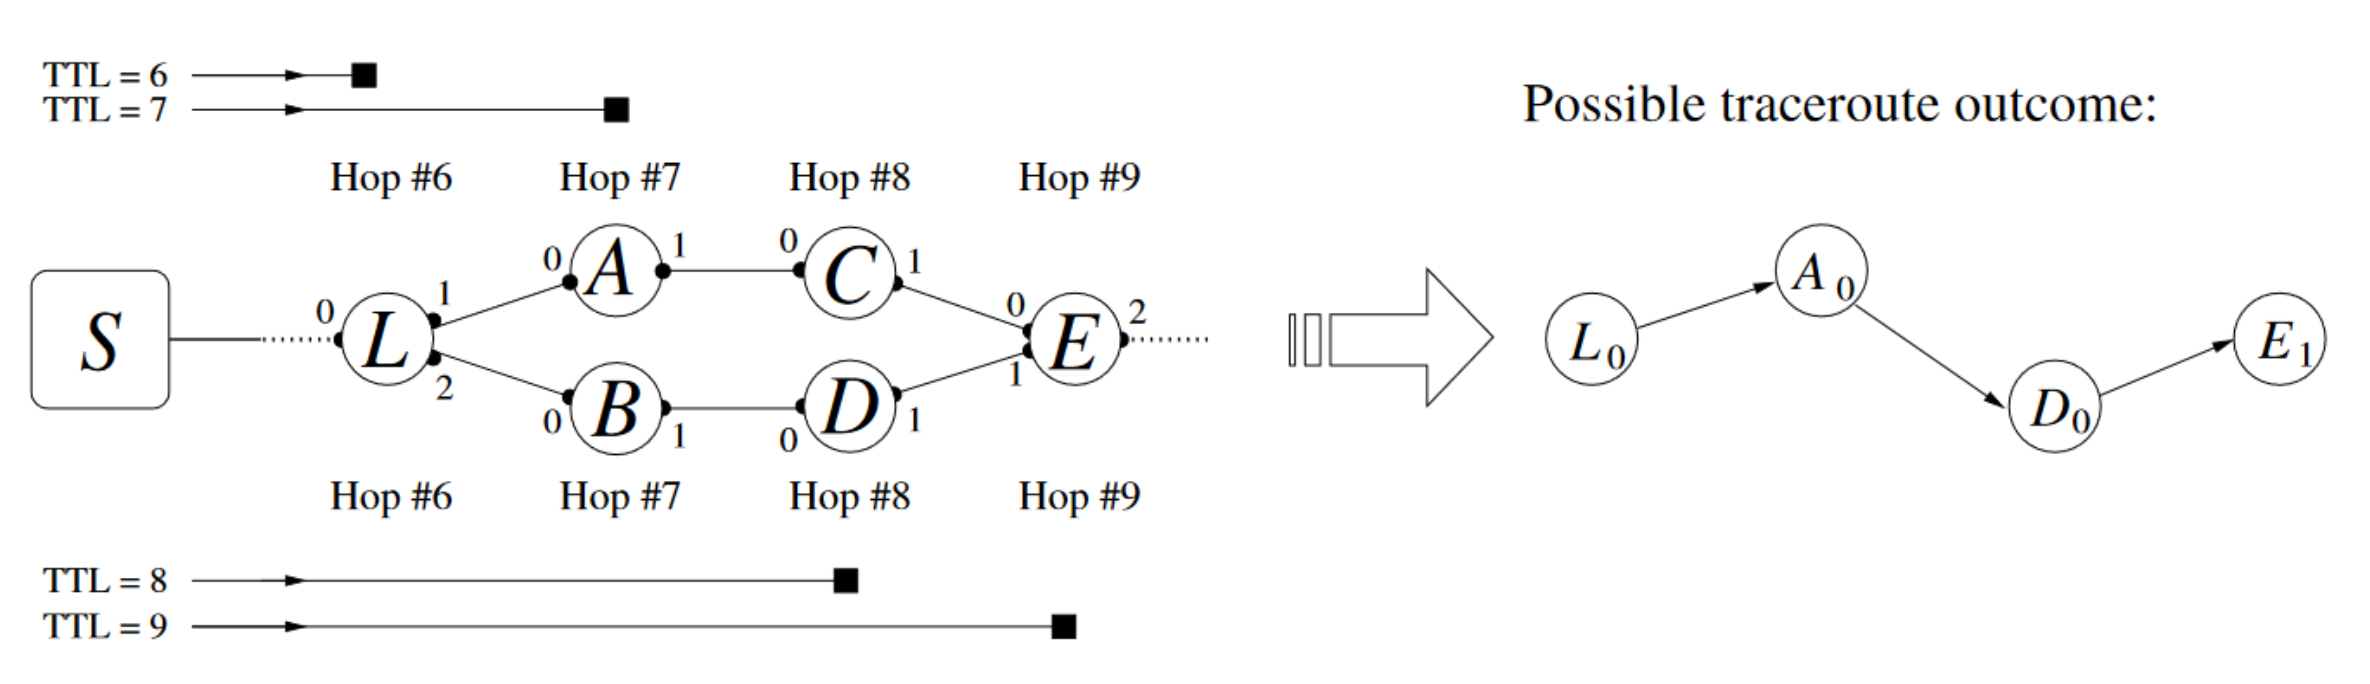
\includegraphics[scale=0.3]{images/missing_nodes.png}
    \caption{Missing nodes and links, and false links \cite{anomalies}}
    \label{figure:missing_node_fig}
  \end{center}
\end{figure}

%----------------------------------------------------
%Different network topology types and their implications

Due to the large prevalence of routers using Load balancing this is highly problematic, in response to this, new approaches have been proposed to mitigate the issue's highlighted above.
%------------------------------------------------------


%Paris trace route
A modern variant of the original traceroute tool called Paris traceroute aims to address the problems posed by networks which employ load-balancing. It does this by manipulating the probe packet header fields, such that all probes follow the same path for per flow load balancing. However, due to probes being sent randomly in a network which uses per packet load balancing, Paris traceroute is unable to perfectly determine all paths in this instance. 
Additionally, it can detect the type of load balancing is being utilized by the network. The can aid diagnostics and help flag instances of potentially wrong mapped routes. \cite{anomalies}

\begin{figure}[!ht]
  \begin{center}
    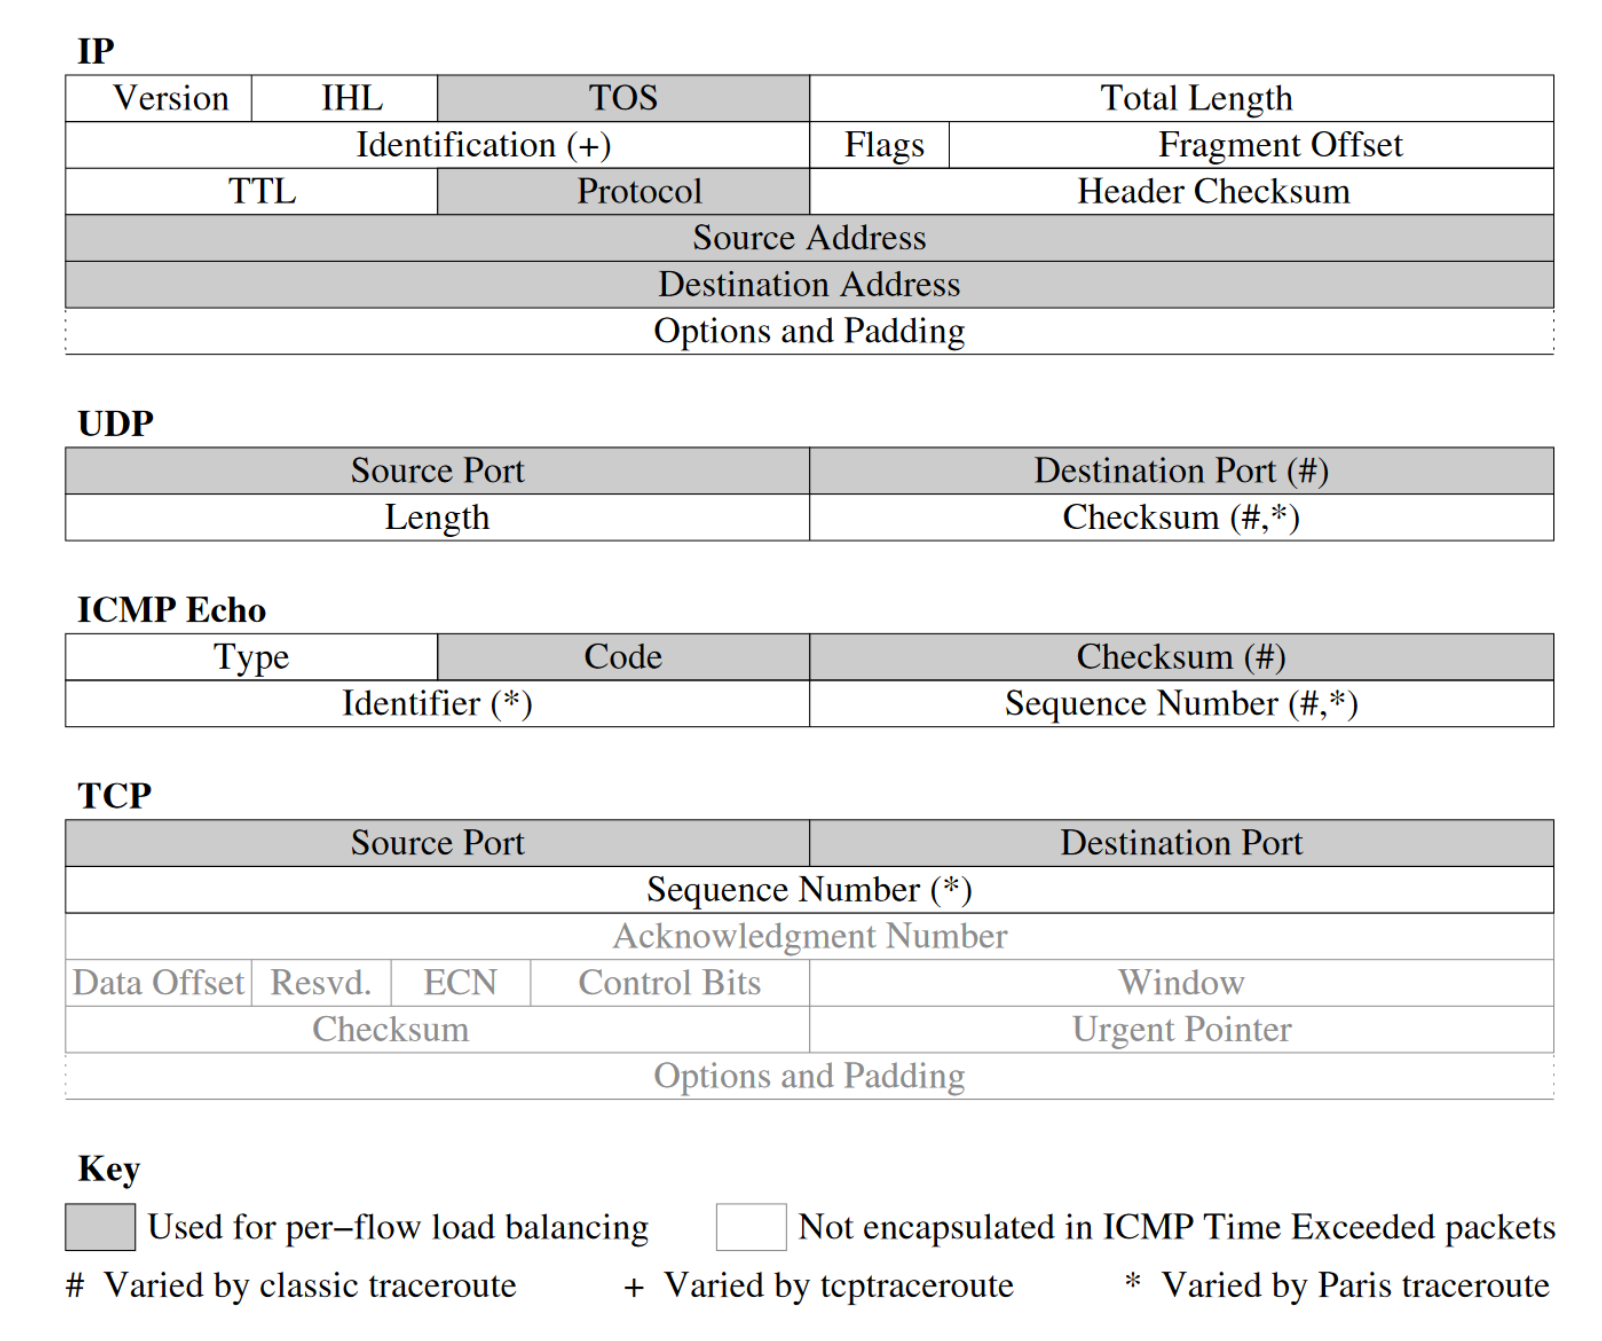
\includegraphics[scale=0.3]{images/packet_header.png}
    \caption{The roles played by packet header fields \cite{anomalies}}
    \label{figure:packet_header_fig}
  \end{center}
\end{figure}

%Analysis
Paris traceroute is a much more robust tool to map internet topology than traceroute as it can mitigate the effects of per-flow load balancing and ensure packets flow on the correct path through the network nodes, avoiding potential missing nodes/links and false links. However, nodes which use Network Address Translation(NAT) can still be problematic for paris traceroute due to the NAT modifying the source/destination IP addresses in the packet headers, obscuring the packet information and also therefore the actual routing path. \cite{anomalies}

%-------------------------------------------------------
%MDA
Further improvements have been made built upon the Paris traceroute tool such as the Multi path Detection Algorithm (MDA). The MDA "provides an extension to Paris traceroute called the MDA, a stochastic probing algorithm that adapts the number of
probes to send on a hop-by-hop basis in order to enumerate all reachable interfaces at each hop". \cite{MDA2}

%Analysis
Rather than send a set amount of probes per hop like the original traceroute which sends 3, the MDA varies this amount based on a controllable parameter. \cite{MDA2} The parameter is the upper limit of the probability of not revealing the entire multi-path network. This is highly advantageous as it can adapt to any given network structure, which in the "real" internet can be extremely complex and have many paths, but also due to it's adaptability it can still remain relatively lightweight. However, as it is a stochastic algorithm there is an element of uncertainty to the produced result, this is accounted for by "yeilding" the  confidence of the final output to provide some further information about the validity of the result. \cite{MDA-lite}\cite{diamond-miner}\cite{MDA3}

%Analysis
MDA-lite is a further improvement on the MDA algorithm by reducing overhead, whilst still having the same performance. It achieves this by operating based on the assumption of uniform hops, with probes being sent at each hop without node control, although node control is still employed in specific cases. One flow identifier from each previously discovered vertex in the preceding hop are reused, this is then followed on with further previously used and new flow identifiers. MDA-lite acts on the premise that diamonds which are met during the network scan "will be uniform and un-meshed". \cite{MDA-lite} 

Due to the possibility of these assumptions not actualizing; "MDA-lite tests for a lack of uniformity and the presence of meshing". \cite{MDA-lite} 

If a scanned diamond is not consistent with the prior assumptions the MDA-lite reverts back to the original MDA algorithm. 

\begin{figure}[!ht]
  \begin{center}
    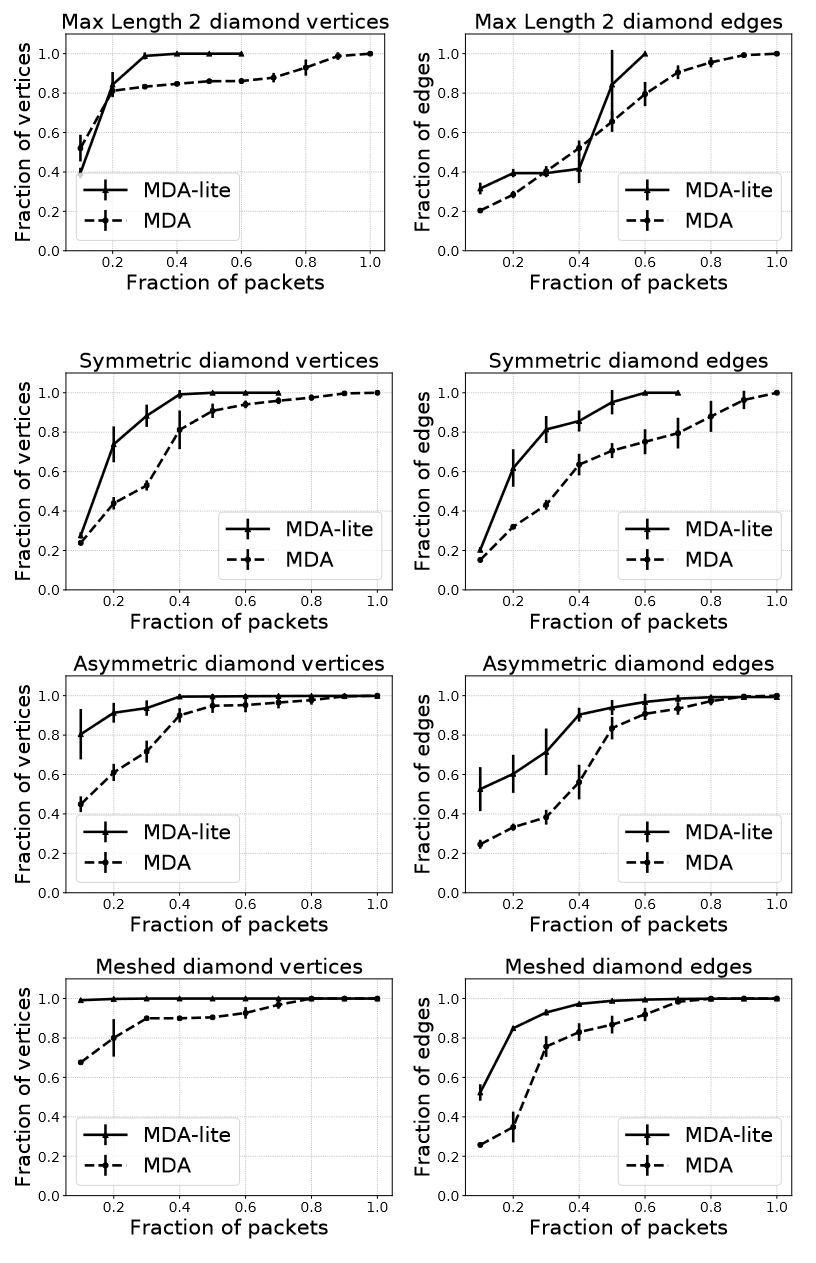
\includegraphics[scale=0.3]{images/MDA_lite.png}
    \caption{MDA-Lite versus MDA simulations\cite{MDA-lite}}
    \label{figure:MDA_lite_fig}
  \end{center}
\end{figure}

%-------------------------------------------------------
%Diamond miner
Another contemporary approach to map network topology is called Diamond Miner, "[it] is designed to capture Internet topology snapshots inclusive of all load-balanced paths". \cite{diamond-miner} Diamond miner utilises Yarrps's randomized and stateless probing, achieving wide coverage of internet topology. Yarrp enables high speed collection of network topology data, due to it's stateless operation and randomization of the probing order of the domain of network ranges and TTL of ICMP packets sent. \cite{yarrp}

\begin{figure}[!ht]
  \begin{center}
    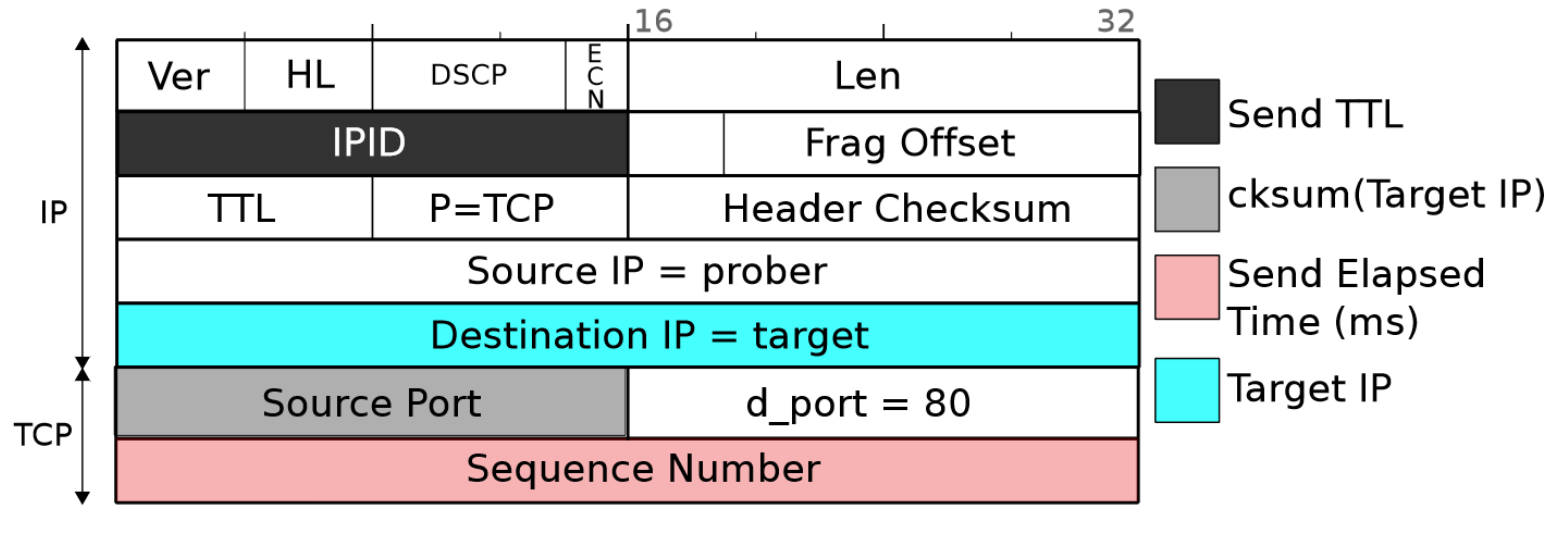
\includegraphics[scale=0.3]{images/yarrp.png}
    \caption{Yarrp encodes information in the IP and TCP field of outgoing proe packets in order to permit stateless operation \cite{yarrp}}
    \label{figure:yarrp_fig}
  \end{center}
\end{figure}

Furthermore, it also incorporates probe set generation logic, which allows tracking of all outbound load-balanced edges from each node with a high certainty. The framework directs Yarrp through multiple iterations, until an adequate discovery level has been achieved for almost every node in the network. \cite{diamond-miner}

\begin{figure}[!ht]
  \begin{center}
    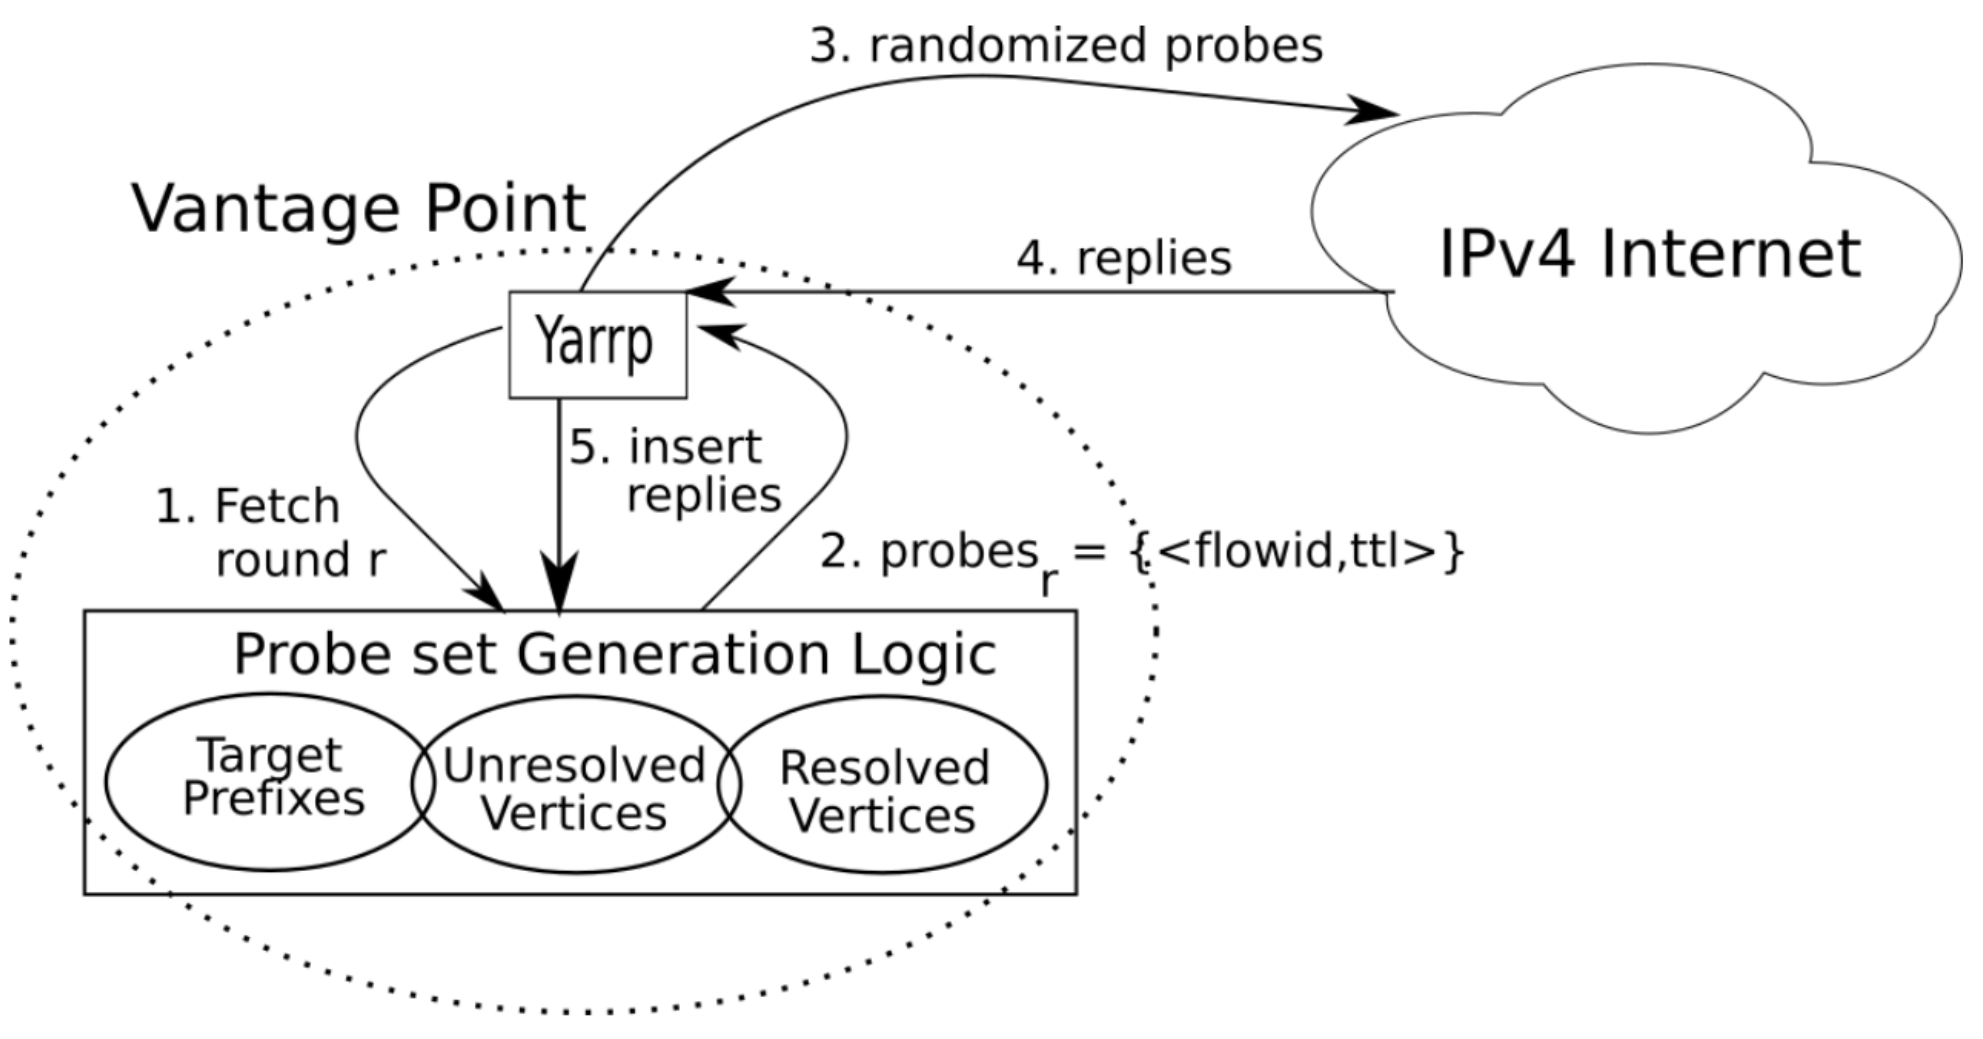
\includegraphics[scale=0.3]{images/diamond.png}
    \caption{Diamond miner high-level conceptual overview \cite{diamond-miner}}
    \label{figure:dminer_overview_fig}
  \end{center}
\end{figure}

%-------------------------------------------------------
%Dublin traceroute
Another modern tool inspired by the original Traceroute, and which builds upon the progress made by Paris traceroute is Dublin Traceroute. Dublin traceroute solves the NAT problem which was a limitation of paris-traceroute."Dublin Traceroute forges a custom IP ID in the outgoing packets, and keeps track of them in the response packets. If the response packet references an outgoing packet with different source/destination IP addresses and ports, this may indicate the presence of a NAT." \cite{dublin} \cite{dublin_website} It is also implemented in C++ for it's core and has also improved on other limitations of Paris traceroute, namely it's memory safety \cite{dublin}, therefore increasing it's robustness. Furthermore, it also offers a python library and interface as a wrapper on top of the C++ codebase. Results are exported as JSON data allowing ease of integration within other applications, adding to it's modularity and usability. \cite{dublin_website}

%--------------------------------------------------------
%Zeph map alogrithms
%Analysis 
By applying reinforcement learning for distributed tracing of network routes, the Zeph algorithmn discovers the probing directives to allocate to the vantages points in order to maximize topology discovery. It follows a sequence of cycles, utilising positive feedback from previous cycles so as to re-enforce the learning process, whilst still trying new directives simultaneously. By using this approach, the total coverage should improve with each continual cycle. \cite{zephMap}

%----------------------------
%2. Can randomly generated topologies capture the characteristics and layout of real-world topologies? 
Given the multitude of tools designed to map internet topologies, an appropriate testing environment should be established to verify the performance of such tools. The need for such an environment is ever increasing, due to the rising complexity of internet networks which can be problematic for scanning tools to operate effectively in. 

"Virtual laboratories are computer-based, interactive environments that allow a user to perform a set of tasks that would normally be performed in a laboratory" \cite{india_virtual}
Utilising a computer-based environment instead of a traditional physical laboratory has utility across many areas of research and science, as it is an effectively "closed" environment from external factors; however, admittedly there are still physical complications that could occur, in the form of "bugs" or electrical faults however these are limited. It also often has a significantly lower overhead, requiring only a computer with a suitable internet connection to replicate complex and varied experimental scenarios. Somewhat obviously, the utility and suitability is more greatly amplified of using a virtual laboratory in the field of computer science. This is due to the subject of measurement or investigation often already existing within a virtual framework, such as a software process within an operating system. However, the study of larger systems consisting of unusual or many sub-systems adds an additional layer of complexity which requires further consideration. One such system is an internet network, which is composed of many nodes and clients interconnected using potentially many different protocols. In an internet network context, a virtual lab can be utilized as a medium in which measurement, observation and management of a simulated network can be accomplished. \cite{virtual_network_lab} 

To successfully capture the complex structure and behaviour of a network, containers can be employed; such as in the case of the containerlab \cite{containerlab} which leverages the docker framework \cite{docker.com}. "The container gives you a “view” or a “slice” of an OS already running. You access OS constructs as if you were running an application directly on the OS". \cite{containerization} Routers and clients can be hosted on discrete containers, which contain their respective operating systems, and then interlinked through configurable protocols. These containers can be interfaced with via SSH or through the docker exec function, enabling interaction from any point in the network. 

%3. What purpose does randomly generating networks which emulate real-world networks fulfil? 
Randomly generated topology structures can be used to augment the diversity of configurations implemented inside a virtual network lab, and also serve as possible benchmarks with which to evaluate contemprary methods and tool. \cite{random_power_grid_topo} Such methods have been suggested by Hoger et al for evaluation of smart grid applications, however there is a gap in the literature evaluating the role that randomly generated networks could serve in an internet network context. 
\begin{figure}
    \centering
    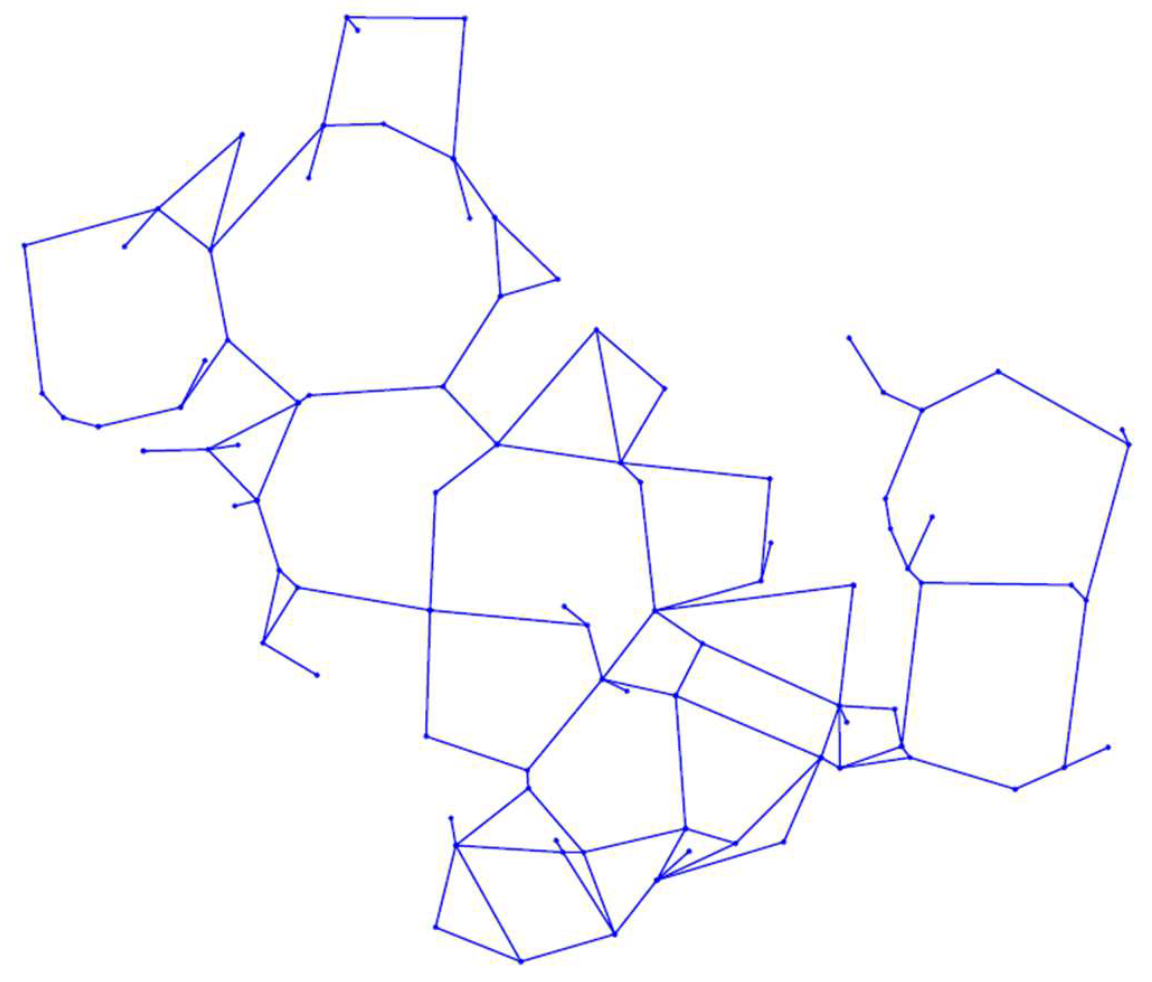
\includegraphics[width=0.5\linewidth]{images/lit_review_top.png}
    \caption{Randomly generated topology designed to replicate power grid networks \cite{random_power_grid_topo}}
    \label{fig:enter-label}
\end{figure}


%4. What is the role of generated network topologies which are different/uncorrelated to real-world networks?

\newpage